\documentclass[italian,12pt]{article}
\usepackage{babel}
\usepackage{amssymb}
\usepackage{amsmath}
\usepackage{graphicx}

\thispagestyle{empty}
\setlength{\textwidth}{18.5cm}
\setlength{\topmargin}{-2.5cm}
\setlength{\textheight}{24.5cm}
\setlength{\oddsidemargin}{-1cm}
\setlength{\evensidemargin}{-1cm}
\begin{document}
\begin{center}{\LARGE Prima prova parziale di Programmazione I}\\
\begin{center}
  \Large 4 febbraio 2013 (tempo disponibile: 2 ore)
\end{center}
\end{center}
%\mbox{}\\
\begin{center}{\Large Esercizio 1}\\
($10$ punti)
\end{center}
Si scriva una funzione
\begin{verbatim}
  double pi(int precision)
\end{verbatim}
che restituisce un'approssimazione di $\pi$ calcolata come:
\[
  \sum\limits_{k=0}^{\mathtt{precision}}\frac{1}{16^k}\left(
    \frac{4}{8k+1}
    -\frac{2}{8k+4}
    -\frac{1}{8k+5}
    -\frac{1}{8k+6}
  \right)
\]

\noindent
Si scriva quindi un \texttt{main} che chiede all'utente la precisione e stampa l'approssimazione
di $\pi$ calcolata con la precedente formula e la precisione inserita, usando 30 cifre
decimali dopo la virgola. Per esempio, una possibile
esecuzione di tale programma potrebbe essere:
%
{\small
\begin{verbatim}
$ ./a.out
precisione: 6
3.141592653228087783645605668426
\end{verbatim}
}
%
\begin{center}{\Large Esercizio 2}\\
($10$ punti)
\end{center}
%
Si scriva una funzione
%
\begin{verbatim}
  void pack(int array[], int length)
\end{verbatim}
%
che riceve come parametri un array di lunghezza pari
\texttt{length} e modifica
l'array in modo che la sua prima met\`a diventi la
somma degli elementi dell'array, due a due, come nel seguente
disegno:

\begin{center}
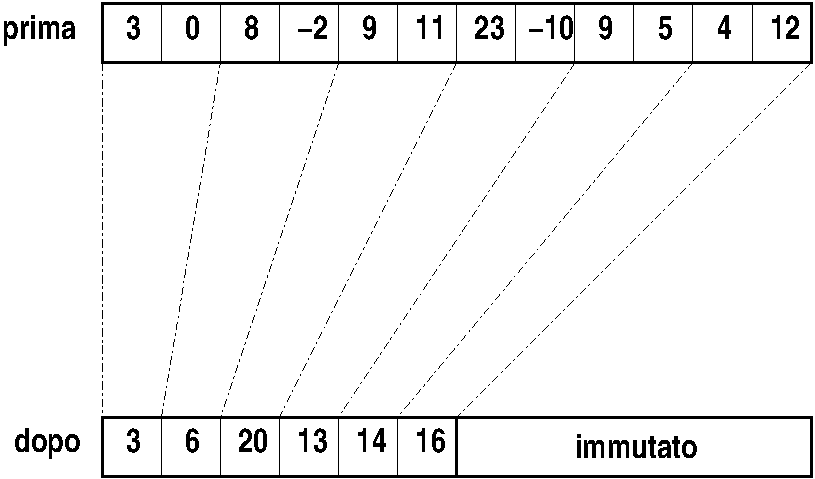
\includegraphics[scale=0.8]{array.pdf}
\end{center}

\newpage
Se tutto \`e corretto, l'esecuzione del seguente \texttt{main}:
{\small
\begin{verbatim}
int main(void) {
  int a[] = { 3, 0, 8, -2, 9, 11, 23, -10, 9, 5, 4, 12 };
  int pos;

  pack(a, 12);

  for (pos = 0; pos < 6; pos++)
    printf("%i ", a[pos]);

  printf("\n");

  return 0;
}
\end{verbatim}
}

\noindent
stamper\`a
%
{\small
\begin{verbatim}
3 6 20 13 14 16
\end{verbatim}
}
%
\begin{center}{\Large Esercizio 3}\\
($12$ punti)\end{center}
%
Si scriva un programma \texttt{cifra\_massima.c} che definisce la funzione ricorsiva
\begin{verbatim}
  int cifra_massima(int num)
\end{verbatim}
%
la quale deve restituire la cifra massima nella rappresentazione decimale di \texttt{num}.
Tale programma dovr\`a inoltre definire un \texttt{main} che chiede all'utente di inserire un numero
non negativo e ne calcola e stampa quindi la cifra massima usando la funzione precedentemente definita.
Per esempio, una possibile esecuzione del programma potrebbe essere:
%
{\small
\begin{verbatim}
$ ./a.out
Inserisci un numero non negativo: 1232 
La cifra massima di 1232 e' 3

$ ./a.out
Inserisci un numero non negativo: 0
La cifra massima di 0 e' 0

$ ./a.out
Inserisci un numero non negativo: -5
Inserisci un numero non negativo: 30756
La cifra massima di 30756 e' 7
\end{verbatim}
}

\end{document}
